\documentclass{beamer}

% -------------------------
% Theme & Earthy Colors
% -------------------------
\usetheme{Madrid}

\definecolor{EarthGreen}{RGB}{85,107,47}
\definecolor{ClayBrown}{RGB}{150,111,51}
\definecolor{Sand}{RGB}{235,224,205}
\definecolor{DeepOlive}{RGB}{60,75,40}

\setbeamercolor{structure}{fg=EarthGreen}
\setbeamercolor{title}{fg=DeepOlive}
\setbeamercolor{frametitle}{fg=DeepOlive,bg=Sand}
\setbeamercolor{block title}{fg=white,bg=ClayBrown}
\setbeamercolor{block body}{bg=Sand!30}
\setbeamertemplate{navigation symbols}{}

% -------------------------
% Packages
% -------------------------
\usepackage{graphicx}
\usepackage{amsmath}
\usepackage{hyperref}

% -------------------------
% Title
% -------------------------
\title{Statistical Estimation via OLS and MLE}
\author{Liam Whitenack \\ 
DASC 605 \\ 
Professor Trent Buskirk \\ 
Old Dominion University}
\date{\today}

\begin{document}

% -------------------------
\begin{frame}
\titlepage
\end{frame}

% -------------------------
\begin{frame}{Data}
\small
\begin{itemize}
    \item Dataset collected in Fall 2025
    \item Source: \href{https://boardgamegeek.com/wiki/page/BGG_XML_API2}{BoardGameGeek XML API Documentation}
    \item Additional reference: 
    \href{https://boardgamegeek.com/wiki/page/BGG_XML_API?redirectedfrom=XML_API}{BGG API Overview}
    \item Processing code available on 
    \href{https://github.com/LiamWhitenack/board-game-geek.git}{GitHub Repository}
    \item Target variable: Bayesian average rating ($Y$)
    \item Predictors: year published, complexity, playing time, player characteristics
    \item Final sample size: 3,833 games (minimum 1000 ratings)
\end{itemize}
\end{frame}

% -------------------------
\begin{frame}{Research Goal}
\centering
\Large
Estimate the relationship between game characteristics and average rating
\\[0.4cm]
Using a linear regression framework grounded in \textbf{Maximum Likelihood Estimation}
\end{frame}

% -------------------------
\begin{frame}{Statistical Model}

\[
Y_i = \beta_0 + \beta_1 X_{i1} + \dots + \beta_k X_{ik} + \varepsilon_i
\]

\[
\varepsilon_i \sim \mathcal{N}(0, \sigma^2)
\]

\bigskip

Under the normality assumption:

\[
\hat{\beta} = \arg\max_{\beta} L(\beta)
\]

Maximizing the likelihood is equivalent to minimizing squared error.

\[
\Rightarrow \textbf{Ordinary Least Squares}
\]

Thus, OLS is the MLE estimator under Gaussian errors.
\end{frame}

% -------------------------
\begin{frame}{Estimation in Python}

\begin{verbatim}
model = sm.OLS(y, X)
results = model.fit()

print(results.summary())
\end{verbatim}

This implements Ordinary Least Squares, 
which corresponds to the MLE solution under normal errors.
\end{frame}

% -------------------------
\begin{frame}{Pre-Regression Distribution}

\begin{center}
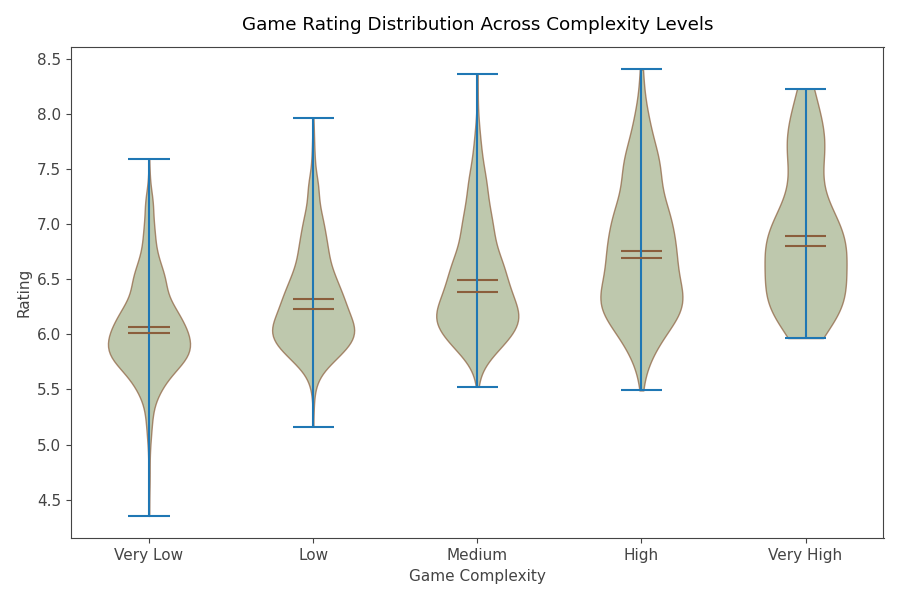
\includegraphics[width=0.8\linewidth]{pre_violin.png}
\end{center}

\end{frame}

% -------------------------
\begin{frame}{OLS Fit}

\begin{center}
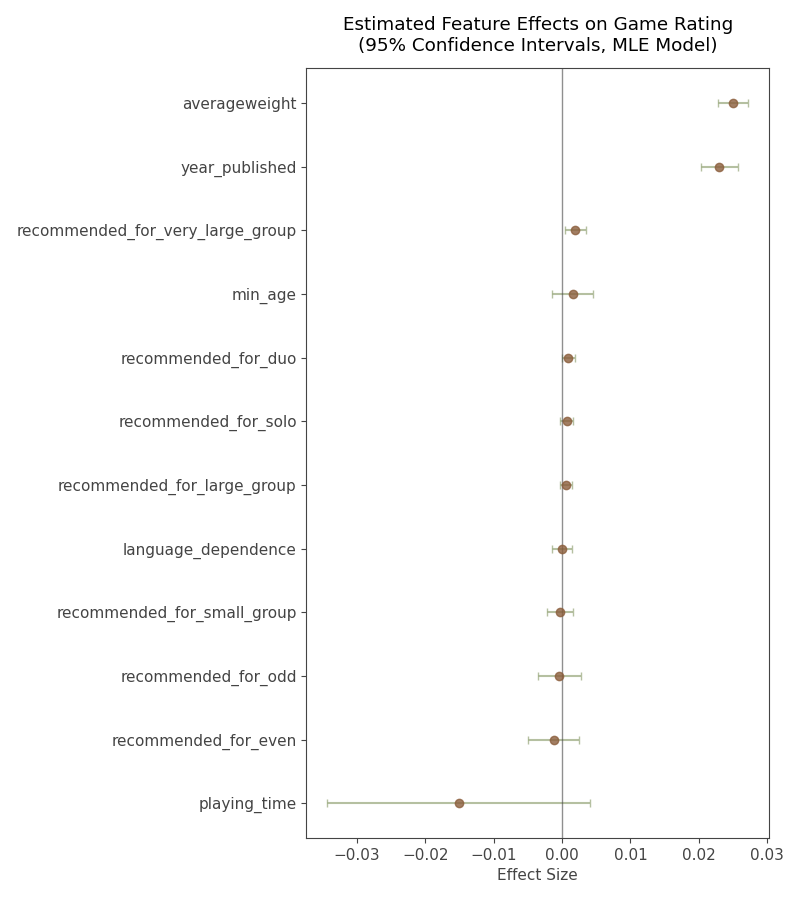
\includegraphics[width=0.6\linewidth]{ols_residuals.png}
\end{center}

\end{frame}

% -------------------------
\begin{frame}{Residual Distribution}

\begin{center}
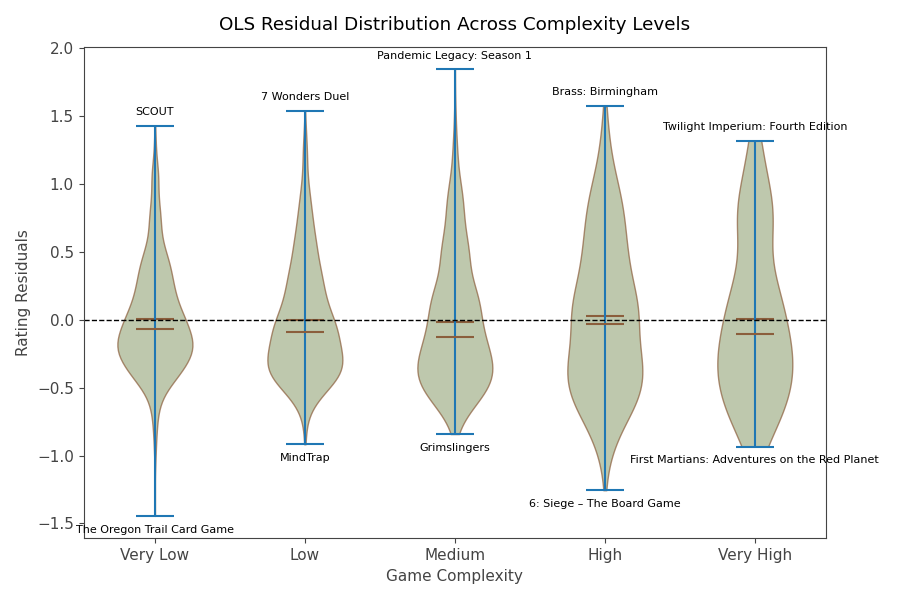
\includegraphics[width=0.8\linewidth]{residual_violin.png}
\end{center}

\end{frame}


\end{document}